\chapter{Licence}

The STLNormalSwitcher is supplied under the terms of the GNU GPL:\\[0.3cm]

\noindent
\copyright 2007 PG500, ISF, University of Dortmund\\
\qquad PG500 are: Christoph Begau, Christoph Heuel, Raffael Joliet, Jan Kolanski, Mandy Kr�ller, Christian Moritz, Daniel Niggemann, Mathias St�ber, Timo St�nner, Jan Varwig, Dafan Zhai\\[0.3cm]

\hspace{0.2\linewidth} GNU GENERAL PUBLIC LICENSE\newline

\hspace{0.3\linewidth} Version 2, June 1991\\

Copyright (C) 1989, 1991 Free Software Foundation, Inc., 51 Franklin Street, Fifth Floor, Boston, MA 02110-1301 USA Everyone is permitted to copy and distribute verbatim copies of this license document, but changing it is not allowed.

\hspace{0.4\linewidth} {\bfseries Preamble}

The licenses for most software are designed to take away your freedom to share and change it. By contrast, the GNU General Public License is intended to guarantee your freedom to share and change free software--to make sure the software is free for all its users.  This General Public License applies to most of the Free Software Foundation's software and to any other program whose authors commit to using it.  (Some other Free Software Foundation software is covered by
the GNU Lesser General Public License instead.)  You can apply it to your programs, too.

When we speak of free software, we are referring to freedom, not price.  Our General Public Licenses are designed to make sure that you have the freedom to distribute copies of free software (and charge for this service if you wish), that you receive source code or can get it if you want it, that you can change the software or use pieces of it in new free programs; and that you know you can do these things.

To protect your rights, we need to make restrictions that forbid anyone to deny you these rights or to ask you to surrender the rights. These restrictions translate to certain responsibilities for you if you distribute copies of the software, or if you modify it.

For example, if you distribute copies of such a program, whether gratis or for a fee, you must give the recipients all the rights that you have. You must make sure that they, too, receive or can get the
source code. And you must show them these terms so they know their rights.

We protect your rights with two steps: (1) copyright the software, and (2) offer you this license which gives you legal permission to copy, distribute and/or modify the software.

Also, for each author's protection and ours, we want to make certain that everyone understands that there is no warranty for this free software.  If the software is modified by someone else and passed on, we want its recipients to know that what they have is not the original, so that any problems introduced by others will not reflect on the original authors' reputations.

Finally, any free program is threatened constantly by software patents.  We wish to avoid the danger that redistributors of a free program will individually obtain patent licenses, in effect making the program proprietary.  To prevent this, we have made it clear that any patent must be licensed for everyone's free use or not licensed at all.

The precise terms and conditions for copying, distribution and modification follow.\\

\hspace{0.2\linewidth} GNU GENERAL PUBLIC LICENSE\\
TERMS AND CONDITIONS FOR COPYING, DISTRIBUTION AND MODIFICATION

\begin{itemize}
	\item[0.] This License applies to any program or other work which contains a notice placed by the copyright holder saying it may be distributed under the terms of this General Public License.  The "Program", below, refers to any such program or work, and a "work based on the Program" means either the Program or any derivative work under copyright law: that is to say, a work containing the Program or a portion of it, either verbatim or with modifications and/or translated into another language.  (Hereinafter, translation is included without limitation in the term "modification".)  Each licensee is addressed as "you".

Activities other than copying, distribution and modification are not covered by this License; they are outside its scope. The act of running the Program is not restricted, and the output from the Program is covered only if its contents constitute a work based on the Program (independent of having been made by running the Program). Whether that is true depends on what the Program does.

  \item[1.] You may copy and distribute verbatim copies of the Program's source code as you receive it, in any medium, provided that you conspicuously and appropriately publish on each copy an appropriate copyright notice and disclaimer of warranty; keep intact all the notices that refer to this License and to the absence of any warranty; and give any other recipients of the Program a copy of this License along with the Program.

You may charge a fee for the physical act of transferring a copy, and you may at your option offer warranty protection in exchange for a fee.

  \item[2.] You may modify your copy or copies of the Program or any portion of it, thus forming a work based on the Program, and copy and distribute such modifications or work under the terms of Section 1 above, provided that you also meet all of these conditions:
		\begin{itemize}
    	\item[a)] You must cause the modified files to carry prominent notices stating that you changed the files and the date of any change.

    	\item[b)] You must cause any work that you distribute or publish, that in whole or in part contains or is derived from the Program or any part thereof, to be licensed as a whole at no charge to all third parties under the terms of this License.

    	\item[c)] If the modified program normally reads commands interactively when run, you must cause it, when started running for such interactive use in the most ordinary way, to print or display an announcement including an appropriate copyright notice and a notice that there is no warranty (or else, saying that you provide a warranty) and that users may redistribute the program under these conditions, and telling the user how to view a copy of this License. (Exception: if the Program itself is interactive but does not normally print such an announcement, your work based on the Program is not required to print an announcement.)
		\end{itemize}
		
These requirements apply to the modified work as a whole.  If identifiable sections of that work are not derived from the Program, and can be reasonably considered independent and separate works in themselves, then this License, and its terms, do not apply to those sections when you distribute them as separate works.  But when you distribute the same sections as part of a whole which is a work based on the Program, the distribution of the whole must be on the terms of this License, whose permissions for other licensees extend to the entire whole, and thus to each and every part regardless of who wrote it.

Thus, it is not the intent of this section to claim rights or contest your rights to work written entirely by you; rather, the intent is to exercise the right to control the distribution of derivative or collective works based on the Program.

In addition, mere aggregation of another work not based on the Program with the Program (or with a work based on the Program) on a volume of a storage or distribution medium does not bring the other work under the scope of this License.

  \item[3.] You may copy and distribute the Program (or a work based on it, under Section 2) in object code or executable form under the terms of Sections 1 and 2 above provided that you also do one of the following:
		\begin{itemize}
    	\item[a)] Accompany it with the complete corresponding machine-readable source code, which must be distributed under the terms of Sections 1 and 2 above on a medium customarily used for software interchange; or,

    	\item[b)] Accompany it with a written offer, valid for at least three years, to give any third party, for a charge no more than your cost of physically performing source distribution, a complete machine-readable copy of the corresponding source code, to be distributed under the terms of Sections 1 and 2 above on a medium customarily used for software interchange; or,

    	\item[c)] Accompany it with the information you received as to the offer to distribute corresponding source code. (This alternative is allowed only for noncommercial distribution and only if you received the program in object code or executable form with such an offer, in accord with Subsection b above.)
		\end{itemize}
The source code for a work means the preferred form of the work for making modifications to it. For an executable work, complete source code means all the source code for all modules it contains, plus any associated interface definition files, plus the scripts used to control compilation and installation of the executable.  However, as a special exception, the source code distributed need not include anything that is normally distributed (in either source or binary form) with the major components (compiler, kernel, and so on) of the operating system on which the executable runs, unless that component itself accompanies the executable.

If distribution of executable or object code is made by offering access to copy from a designated place, then offering equivalent access to copy the source code from the same place counts as distribution of the source code, even though third parties are not compelled to copy the source along with the object code.

  \item[4.] You may not copy, modify, sublicense, or distribute the Program except as expressly provided under this License.  Any attempt otherwise to copy, modify, sublicense or distribute the Program is void, and will automatically terminate your rights under this License. However, parties who have received copies, or rights, from you under this License will not have their licenses terminated so long as such parties remain in full compliance.

  \item[5.] You are not required to accept this License, since you have not signed it.  However, nothing else grants you permission to modify or distribute the Program or its derivative works.  These actions are prohibited by law if you do not accept this License.  Therefore, by modifying or distributing the Program (or any work based on the Program), you indicate your acceptance of this License to do so, and all its terms and conditions for copying, distributing or modifying the Program or works based on it.

  \item[6.] Each time you redistribute the Program (or any work based on the Program), the recipient automatically receives a license from the original licensor to copy, distribute or modify the Program subject to these terms and conditions. You may not impose any further restrictions on the recipients' exercise of the rights granted herein. You are not responsible for enforcing compliance by third parties to this License.

  \item[7.] If, as a consequence of a court judgment or allegation of patent infringement or for any other reason (not limited to patent issues), conditions are imposed on you (whether by court order, agreement or otherwise) that contradict the conditions of this License, they do not excuse you from the conditions of this License. If you cannot distribute so as to satisfy simultaneously your obligations under this License and any other pertinent obligations, then as a consequence you may not distribute the Program at all.  For example, if a patent license would not permit royalty-free redistribution of the Program by all those who receive copies directly or indirectly through you, then the only way you could satisfy both it and this License would be to refrain entirely from distribution of the Program.

If any portion of this section is held invalid or unenforceable under any particular circumstance, the balance of the section is intended to apply and the section as a whole is intended to apply in other circumstances.

It is not the purpose of this section to induce you to infringe any patents or other property right claims or to contest validity of any such claims; this section has the sole purpose of protecting the integrity of the free software distribution system, which is implemented by public license practices.  Many people have made generous contributions to the wide range of software distributed through that system in reliance on consistent application of that system; it is up to the author/donor to decide if he or she is willing to distribute software through any other system and a licensee cannot impose that choice.

This section is intended to make thoroughly clear what is believed to be a consequence of the rest of this License.

  \item[8.] If the distribution and/or use of the Program is restricted in certain countries either by patents or by copyrighted interfaces, the original copyright holder who places the Program under this License may add an explicit geographical distribution limitation excluding those countries, so that distribution is permitted only in or among countries not thus excluded.  In such case, this License incorporates the limitation as if written in the body of this License.

  \item[9.] The Free Software Foundation may publish revised and/or new versions of the General Public License from time to time.  Such new versions will be similar in spirit to the present version, but may differ in detail to address new problems or concerns.

Each version is given a distinguishing version number.  If the Program specifies a version number of this License which applies to it and "any later version", you have the option of following the terms and conditions either of that version or of any later version published by the Free Software Foundation.  If the Program does not specify a version number of this License, you may choose any version ever published by the Free Software Foundation.

  \item[10.] If you wish to incorporate parts of the Program into other free programs whose distribution conditions are different, write to the author to ask for permission.  For software which is copyrighted by the Free Software Foundation, write to the Free Software Foundation; we sometimes make exceptions for this.  Our decision will be guided by the two goals of preserving the free status of all derivatives of our free software and of promoting the sharing and reuse of software generally.
\end{itemize}

\hspace{0.3\linewidth} NO WARRANTY

\begin{itemize}
  \item[11.] BECAUSE THE PROGRAM IS LICENSED FREE OF CHARGE, THERE IS NO WARRANTY FOR THE PROGRAM, TO THE EXTENT PERMITTED BY APPLICABLE LAW.  EXCEPT WHEN OTHERWISE STATED IN WRITING THE COPYRIGHT HOLDERS AND/OR OTHER PARTIES PROVIDE THE PROGRAM "AS IS" WITHOUT WARRANTY OF ANY KIND, EITHER EXPRESSED OR IMPLIED, INCLUDING, BUT NOT LIMITED TO, THE IMPLIED WARRANTIES OF MERCHANTABILITY AND FITNESS FOR A PARTICULAR PURPOSE.  THE ENTIRE RISK AS TO THE QUALITY AND PERFORMANCE OF THE PROGRAM IS WITH YOU.  SHOULD THE PROGRAM PROVE DEFECTIVE, YOU ASSUME THE COST OF ALL NECESSARY SERVICING, REPAIR OR CORRECTION.

  \item[12.] IN NO EVENT UNLESS REQUIRED BY APPLICABLE LAW OR AGREED TO IN WRITING WILL ANY COPYRIGHT HOLDER, OR ANY OTHER PARTY WHO MAY MODIFY AND/OR REDISTRIBUTE THE PROGRAM AS PERMITTED ABOVE, BE LIABLE TO YOU FOR DAMAGES, INCLUDING ANY GENERAL, SPECIAL, INCIDENTAL OR CONSEQUENTIAL DAMAGES ARISING OUT OF THE USE OR INABILITY TO USE THE PROGRAM (INCLUDING BUT NOT LIMITED TO LOSS OF DATA OR DATA BEING RENDERED INACCURATE OR LOSSES SUSTAINED BY YOU OR THIRD PARTIES OR A FAILURE OF THE PROGRAM TO OPERATE WITH ANY OTHER PROGRAMS), EVEN IF SUCH HOLDER OR OTHER PARTY HAS BEEN ADVISED OF THE POSSIBILITY OF SUCH DAMAGES.
\end{itemize}

\qquad\qquad END OF TERMS AND CONDITIONS

\newpage
\noindent
The TAO framework librarys included in this program are supplied under the terms of the MIT-licence:\\[0.3cm]

\noindent
\copyright 2007 The Tao Framework\\[0.3cm]

\noindent
Permission is hereby granted, free of charge, to any person obtaining a copy of this software and
associated documentation files (the "`Software"'), to deal in the Software without restriction,
including without limitation the rights to use, copy, modify, merge, publish, distribute, sublicense,
and/or sell copies of the Software, and to permit persons to whom the Software is furnished to do so,
subject to the following conditions:\\[0.3cm]

\noindent
The above copyright notice and this permission notice shall be included in all copies or substantial portions of the Software.\\[0.2cm]

\noindent
THE SOFTWARE IS PROVIDED "`AS IS"', WITHOUT WARRANTY OF ANY KIND, EXPRESS OR IMPLIED,
INCLUDING BUT NOT LIMITED TO THE WARRANTIES OF MERCHANTABILITY, FITNESS FOR A
PARTICULAR PURPOSE AND NONINFRINGEMENT. IN NO EVENT SHALL THE AUTHORS OR
COPYRIGHT HOLDERS BE LIABLE FOR ANY CLAIM, DAMAGES OR OTHER LIABILITY,
WHETHER IN AN ACTION OF CONTRACT, TORT OR OTHERWISE, ARISING FROM, OUT OF OR
IN CONNECTION WITH THE SOFTWARE OR THE USE OR OTHER DEALINGS IN THE SOFTWARE.

\chapter{Introduction}

STLNormalSwitcher is a small program to view STL-files (see chapter \ref{stlFormat}) and to switch the normal vectors of the triangles contained in it. Switching\index{Switching} a normal vector $(x,y,z)$ means to negate the normal vector to $(-x,-y,-z)$, so that it points the opposite way. STL-files opened in STLNormalSwitcher should not contain more than 16777214 triangles for STLNormalSwitcher to work.\\

\noindent
It allows picking the triangles whose normal vectors are to be switched either from a list\index{List} displaying the numerical values or directly in the graphical representation\index{Display-Area}.\\

\noindent
The STLNormalSwitcher can also be used to convert STL-files from ASCII to Binary or vice versa.

\begin{figure}[hb]
	\centering
	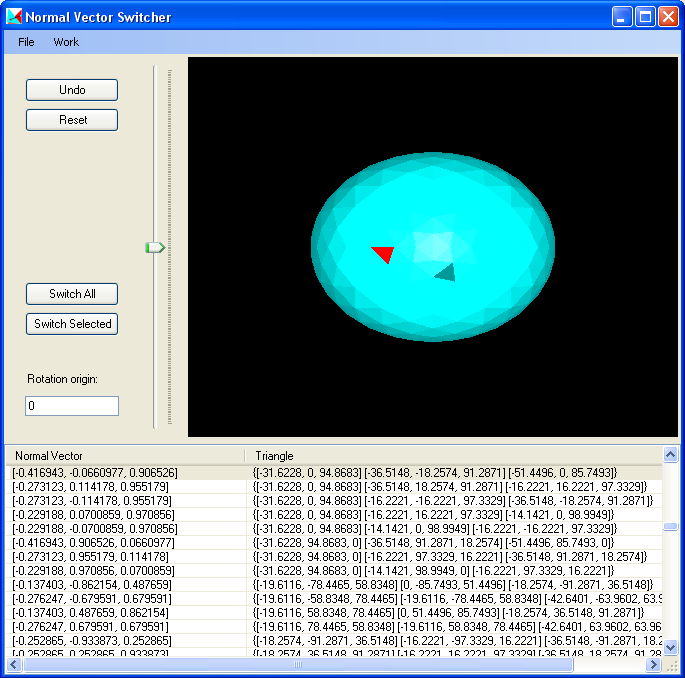
\includegraphics[width=0.70\linewidth]{window1}
\end{figure}


\chapter{The Menu}

\section{The File Menu}

\subsection{Open}
\index{Open}
Closes a previously opened file and opens a new one.\\
The file has to be a valid STL-file\index{STL} (see chapter \ref{stlFormat}).

\subsection{Save}
\index{Save}
Saves changes to the currently opened STL-file in the current format (ASCII or Binary) overwriting the old file.

\subsection{Save As...}
\index{Save As}
Saves changes to the STL-file chosen in the displayed dialogue in the chosen format (ASCII or Binary).

\subsection{Close}
\index{Close}
Closes the current STL-file asking the user whether he wants to save changes and resets the STLNormalSwitcher window.

\subsection{Exit}
\index{Exit}
Ends the program, asking the user to save changes.

\newpage
\section{The Edit Menu}

\subsection{UnDo}
\index{UnDo}
Reverts the last switching operation.

\subsection{Reset}
\index{Reset}
Reverts all switching operations since the STL-file was opened.

\subsection{Switch Selected}
\index{Switching!Selected}
Switches the selected normal vectors.

\subsection{Switch All}
\index{Switching!All}
Switches all normal vectors.


\chapter{The Window}

\section{The Controls}

The buttons "`UnDo"'\index{UnDo}, "`Reset"'\index{Reset}, "`Switch Selected"'\index{Switching!Selected} and "`Switch All"'\index{Switching!All} do just the same as the corresponding menuitems. 

\begin{figure}[hb]
	\centering
	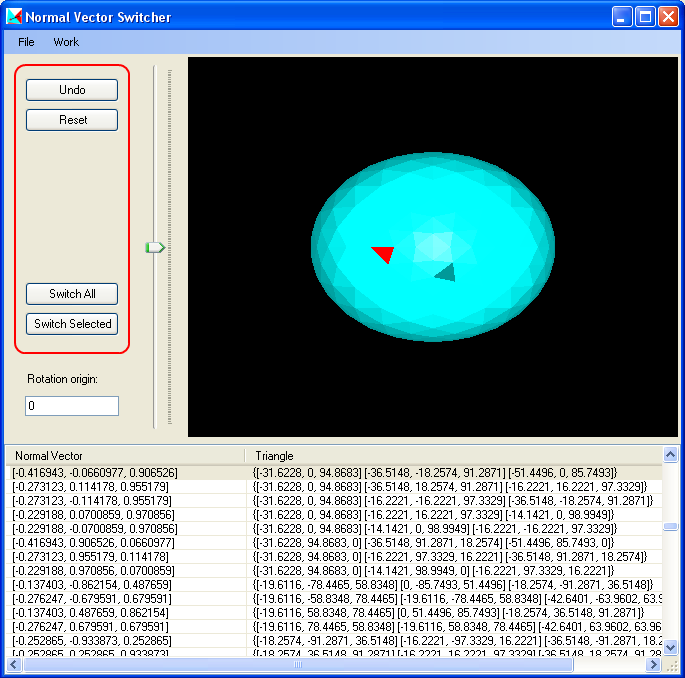
\includegraphics[width=0.9\linewidth]{window2}
\end{figure}

\newpage\noindent
The slider allows a change of the origin of rotation along the z-axis. That value can also be set using the "`Rotation origin"'\index{Rotation Origin} textbox. The value has to be an integer value. The limits for that value will be set according to the values of the vertices in the STL-file\index{STL}. A valid value is accepted when the "`Return-key"' or the "`Enter-key"' is pressed. If the entered value is not valid the rotation origin will be set back to the previous value.

\begin{figure}[hb]
	\centering
	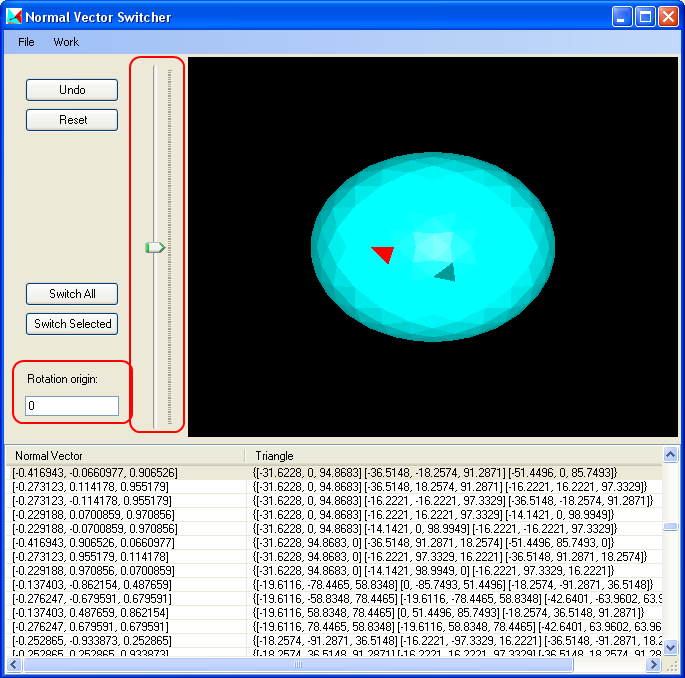
\includegraphics[width=0.9\linewidth]{window3}
\end{figure}

\newpage
\section{The List}

In the list\index{List} at the bottom of the window two columns are displayed. The first column shows the normal vectors and the second column shows the triangles represented by their vertices.
Clicking on a column header will sort the items in the list as strings.
Items can be selected as usual clicking on them using the left mouse button, pulling a rectangle over the left column with the left mouse button pressed to select neighboring items or clicking individual items with the Ctrl-key pressed to selected items that are not direct neighbors.
The selected triangles will be marked red in the Display-Area\index{Display-Area} (see section \ref{displayArea}).

\begin{figure}[hb]
	\centering
	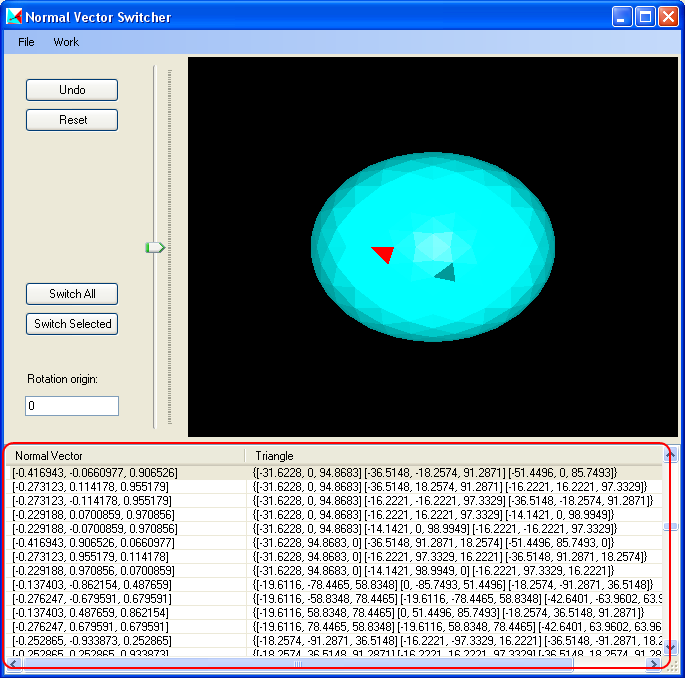
\includegraphics[width=0.9\linewidth]{window4}
\end{figure}

\newpage
\section{The Display-Area}\label{displayArea}

In the Display-Area\index{Display-Area} the workpiece represented in the STL-file\index{STL} is shown. It can be rotated by pressing the right mouse button and dragging the mouse. Zooming is done using the mouse wheel. A single triangle can be picked by clicking it with the left mouse button. Several triangles are picked clicking them with the left mouse button individually and holding down the Ctrl-key. Selected triangles are marked red. Selecting a triangle twice will deselect it. Clicking on the background with the left mouse button will deselect all selected triangles. Triangles with normal vectors pointing away from the viewer can be easily recognised. They don't reflect the light and appear darker as can be seen in the picture below.

\begin{figure}[hb]
	\centering
	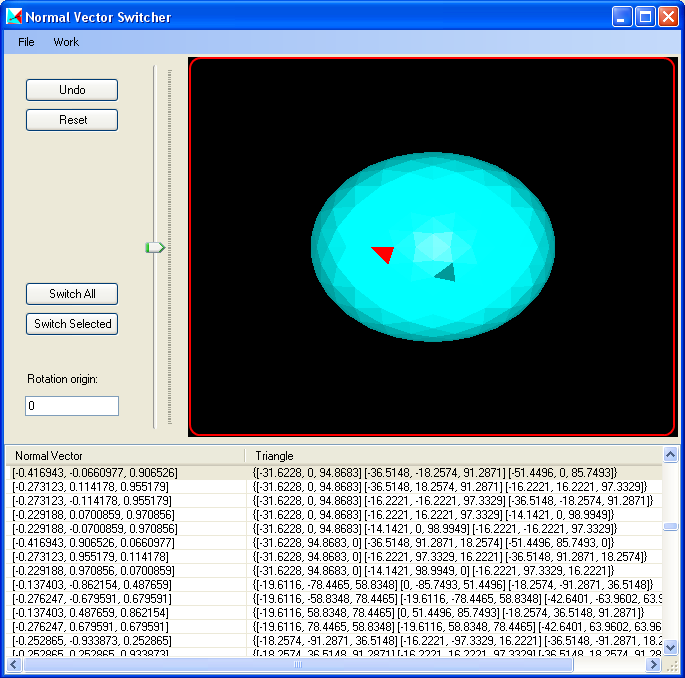
\includegraphics[width=0.9\linewidth]{window5}
\end{figure}


\chapter{STL file format}\label{stlFormat}

STL (SurfaceTesselationLanguage)\index{STL} is a file format native to the stereolithography CAD software created by 3D Systems. This file format is supported by many other software packages. It is widely used for rapid prototyping and computer-aided manufacturing. STL files describe only the surface geometry of a three dimensional object without any representation of color, texture or other common CAD model attributes. The STL format specifies both ASCII and binary representations. Binary files are more common, since they are more compact.

An STL file describes a raw unstructured triangulated surface by the unit normal and vertices of the triangles using a three-dimensional Cartesian coordinate system.


\section{ASCII STL}

An ASCII STL\index{STL!ASCII} file must start with the line:

\begin{verbatim}
	solid name
\end{verbatim}

\noindent
where name is an optional string. The file continues with any number of triangles, each represented as follows:
\begin{verbatim}
 facet normal n1 n2 n3
   outer loop
     vertex v11 v12 v13
     vertex v21 v22 v23
     vertex v31 v32 v33
   endloop
 endfacet
\end{verbatim}

\noindent
and concludes with:

\begin{verbatim}
 endsolid name
\end{verbatim}

\noindent
White space (spaces, tabs, newlines) may be used anywhere in the file except within numbers or words. The spaces between 'facet' and 'normal' and between 'outer' and 'loop' are required.


\section{Binary STL}

Because ASCII STL files can become very large, a binary version of STL \index{STL!Binary} exists. A binary STL file has an 80 character header (Which will be ignored by this program - but should not contain 'vertex' or 'facet'. In contrast to many other programs STLNormalSwitcher can handle headers beginning with 'solid'.). Following the header is a 4 byte unsigned integer indicating the number of triangular facets in the file. Following that is data describing each triangle in turn. The file simply ends after the last triangle.\\

\noindent
Each triangle is described by twelve floating point numbers: three for the normal and then three for the X/Y/Z coordinate of each vertex - just as with the ASCII version of STL. After the twelve floats there is a two byte unsigned 'short' integer that is the 'attribute byte count' - in the standard format, this should be zero because most software does not understand anything else.